\documentclass{beamer}
\usetheme{Goettingen}
\usecolortheme{default}
\usepackage{graphicx}

%\usepackage{times} %For typeface
%\usepackage{epsfig}
\usepackage{color} %For Comments
%\usepackage{beamerthemeshadow} %Paul and Lemmon put this in, take out if you want
%\usepackage{hyperref}
%\usepackage{url}


%% Elena's favorite green (thanks, Fernando!)
\definecolor{ForestGreen}{RGB}{34,139,34}
\definecolor{BlueViolet}{RGB}{138,43,226}
\definecolor{Coquelicot}{RGB}{255, 56, 0}
\definecolor{Teal}{RGB}{2,132,130}
% Uncomment this if you want to show work-in-progress comments
\newcommand{\comment}[1]{{\bf \tt  {#1}}}
% Uncomment this if you don't want to show comments
%\newcommand{\comment}[1]{}
\newcommand{\emcomment}[1]{\textcolor{ForestGreen}{\comment{Elena: {#1}}}}
\newcommand{\todo}[1]{\textcolor{blue}{\comment{To Do: {#1}}}}
%%%%%%%%%%%%%%%%%%%%%%%%%%%%%%%%%%%%%%%%%%

\begin{document}
\title{Developing Beginner-Friendly User Interactions for the Clojure Programming Language}
\author{Richard Stangl, Shamund Gordon, Tony Song, Ben Goldstein}
\institute[UMM] % (optional, but mostly needed)
{
 % \inst{1}%
  University of Minnesota, Morris
}
\date[]  
{HHMI lunch meeting, June 29 2016}

\begin{frame}
  \titlepage
\end{frame}


\begin{frame}

\frametitle{Outline}
\tableofcontents
\end{frame}

\section{Overview of the project}

\begin{frame}
  \frametitle{Overview of the project}
\begin{itemize}
\item Introduction to the project and goals
\item Background information
\end{itemize}
\end{frame}

\begin{frame}
  \frametitle{Introduction to the project and goals}
  ClojureEd
\end{frame}

\begin{frame}
  \frametitle{Background information}
  What is Clojure?
\end{frame}



\section{Usability study}

\begin{frame}
  \frametitle{Usability study}
\begin{itemize}
\item Overview of the usability study 
\item Standard error message vs Modified error message
\item Study procedure
\end{itemize}
\end{frame}

\begin{frame}
  \frametitle{Overview of the Usability Study}
Simply put, the purpose of the study is to compare our modified error messages to standard error messages by lookin at:
\begin{itemize}
\item Success rate
\item Time
\item If not solved, how close or on track were them to solving the question
\end{itemize} 
\end{frame}

\begin{frame}
  \frametitle{Racket Error Messaging}
  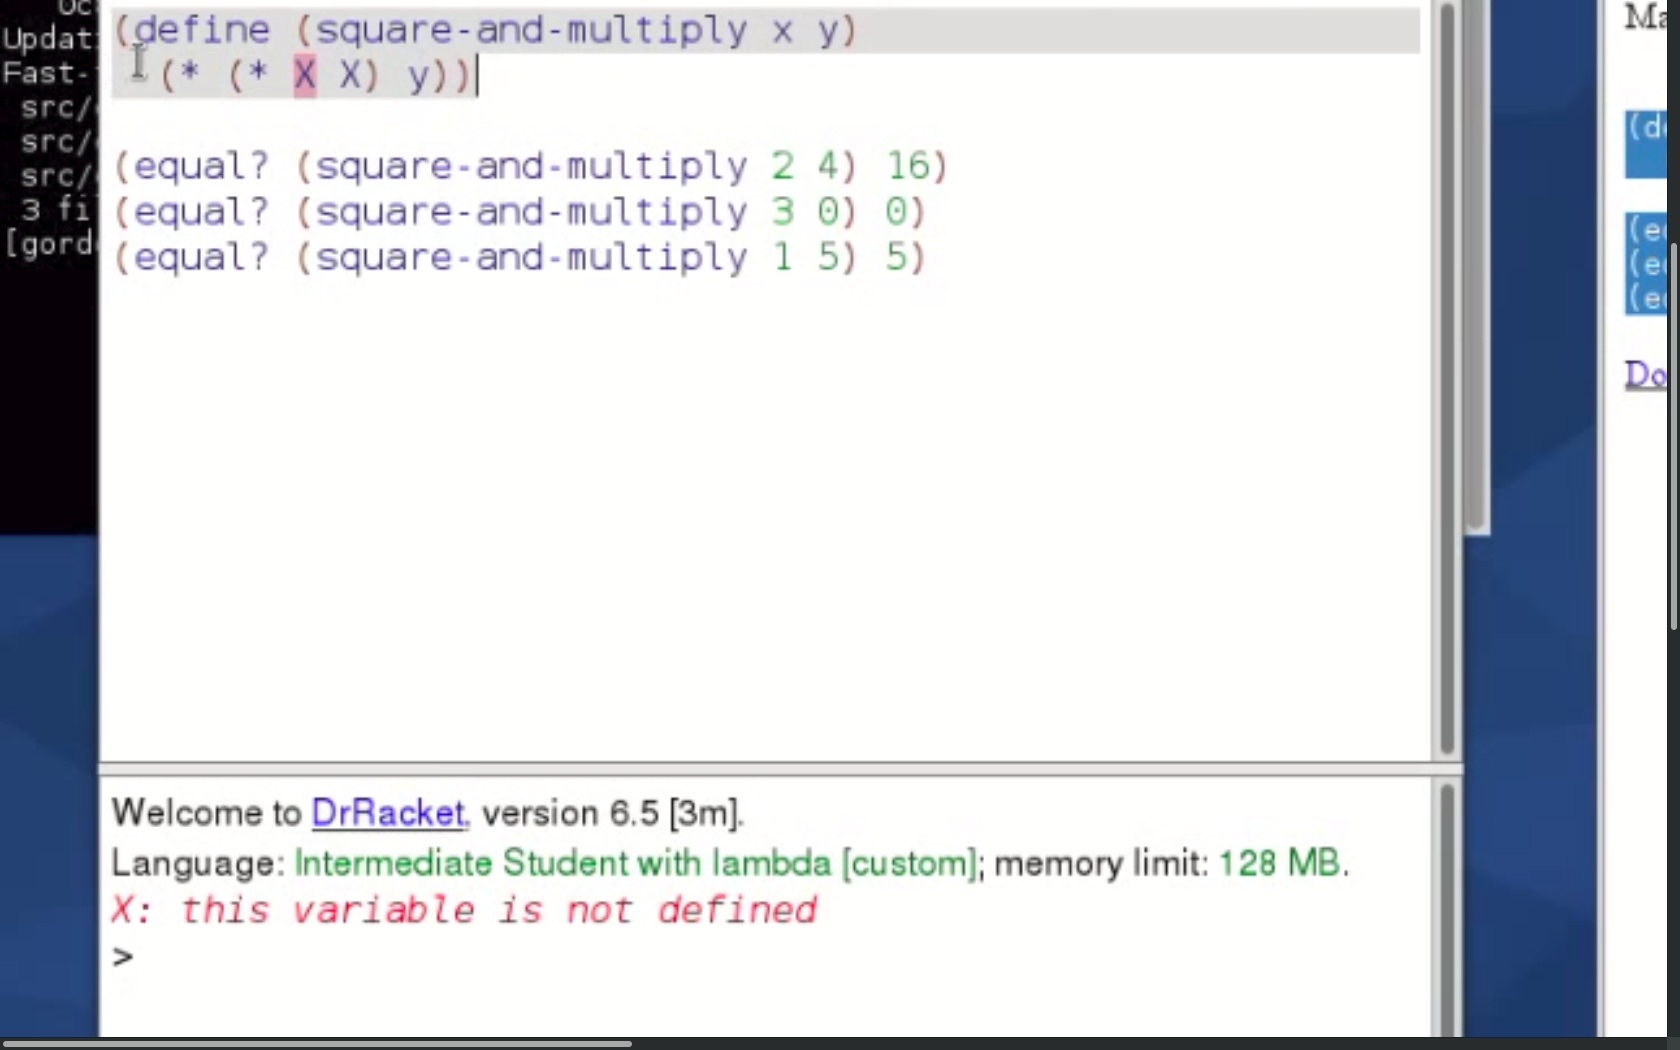
\includegraphics[scale=.17]{R2Rshot}
\end{frame}

\begin{frame}
  \frametitle{Clojure Standard Error Messaging}
  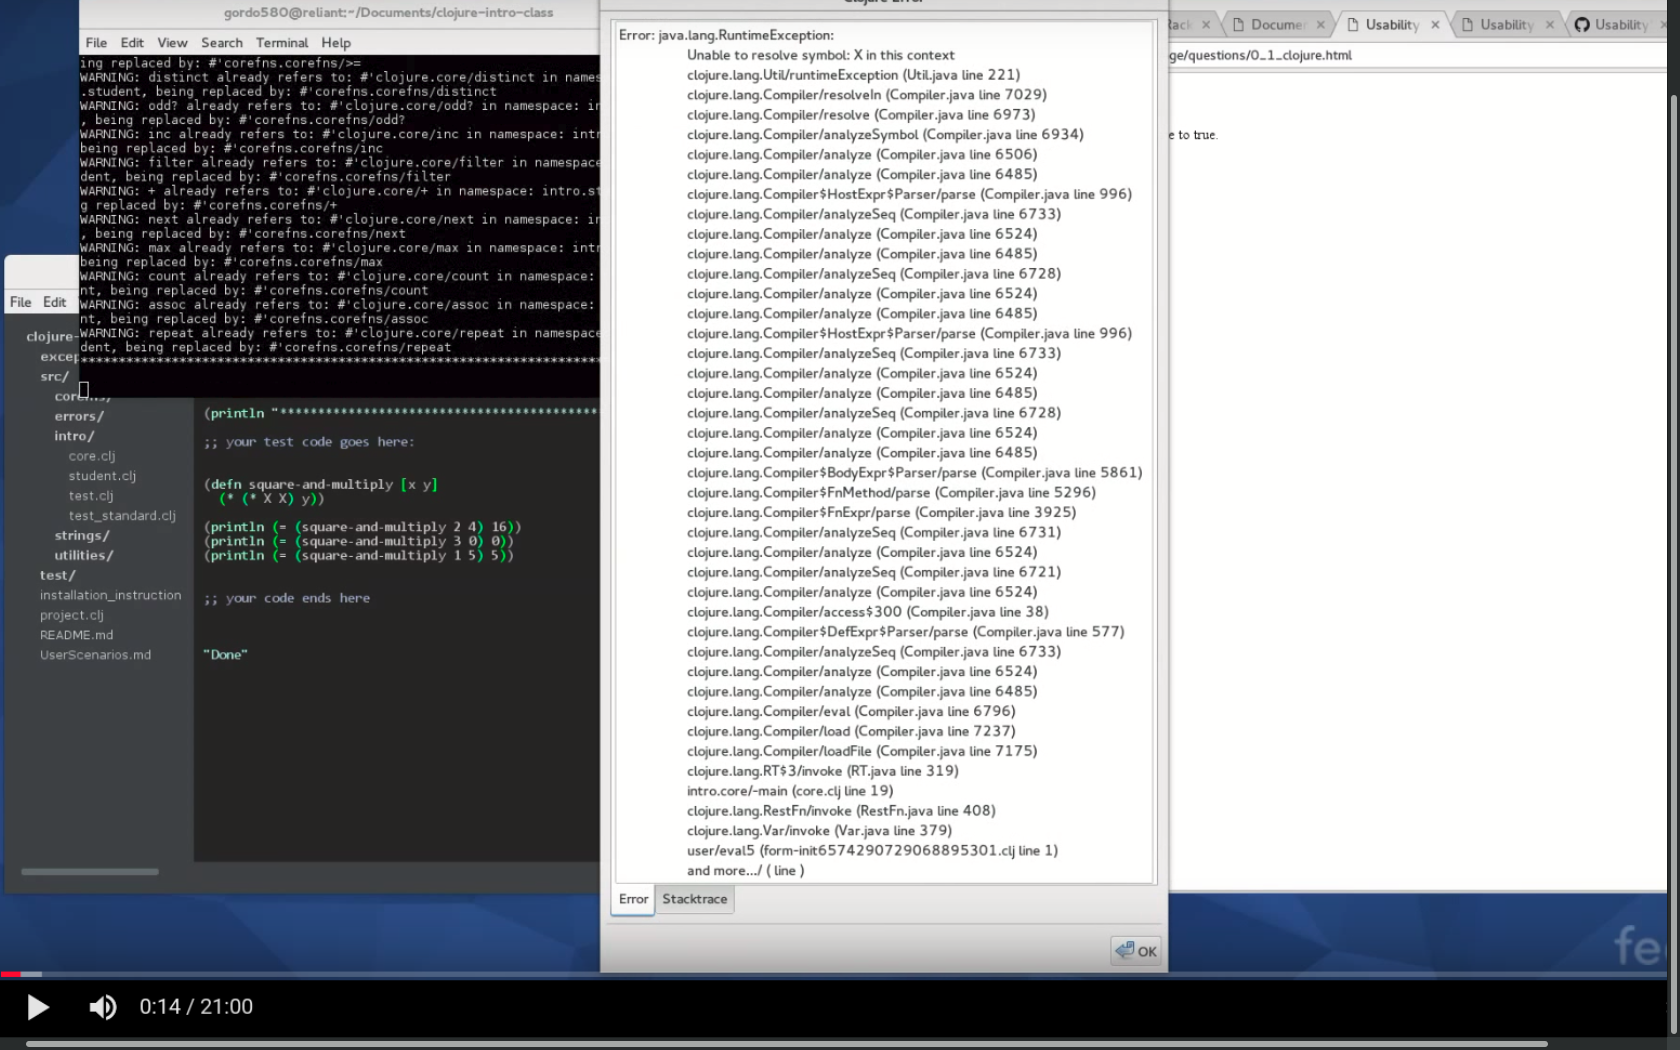
\includegraphics[scale=.17]{CS20Sshot}
\end{frame}

\begin{frame}
  \frametitle{Clojure Modified Error Messaging}
  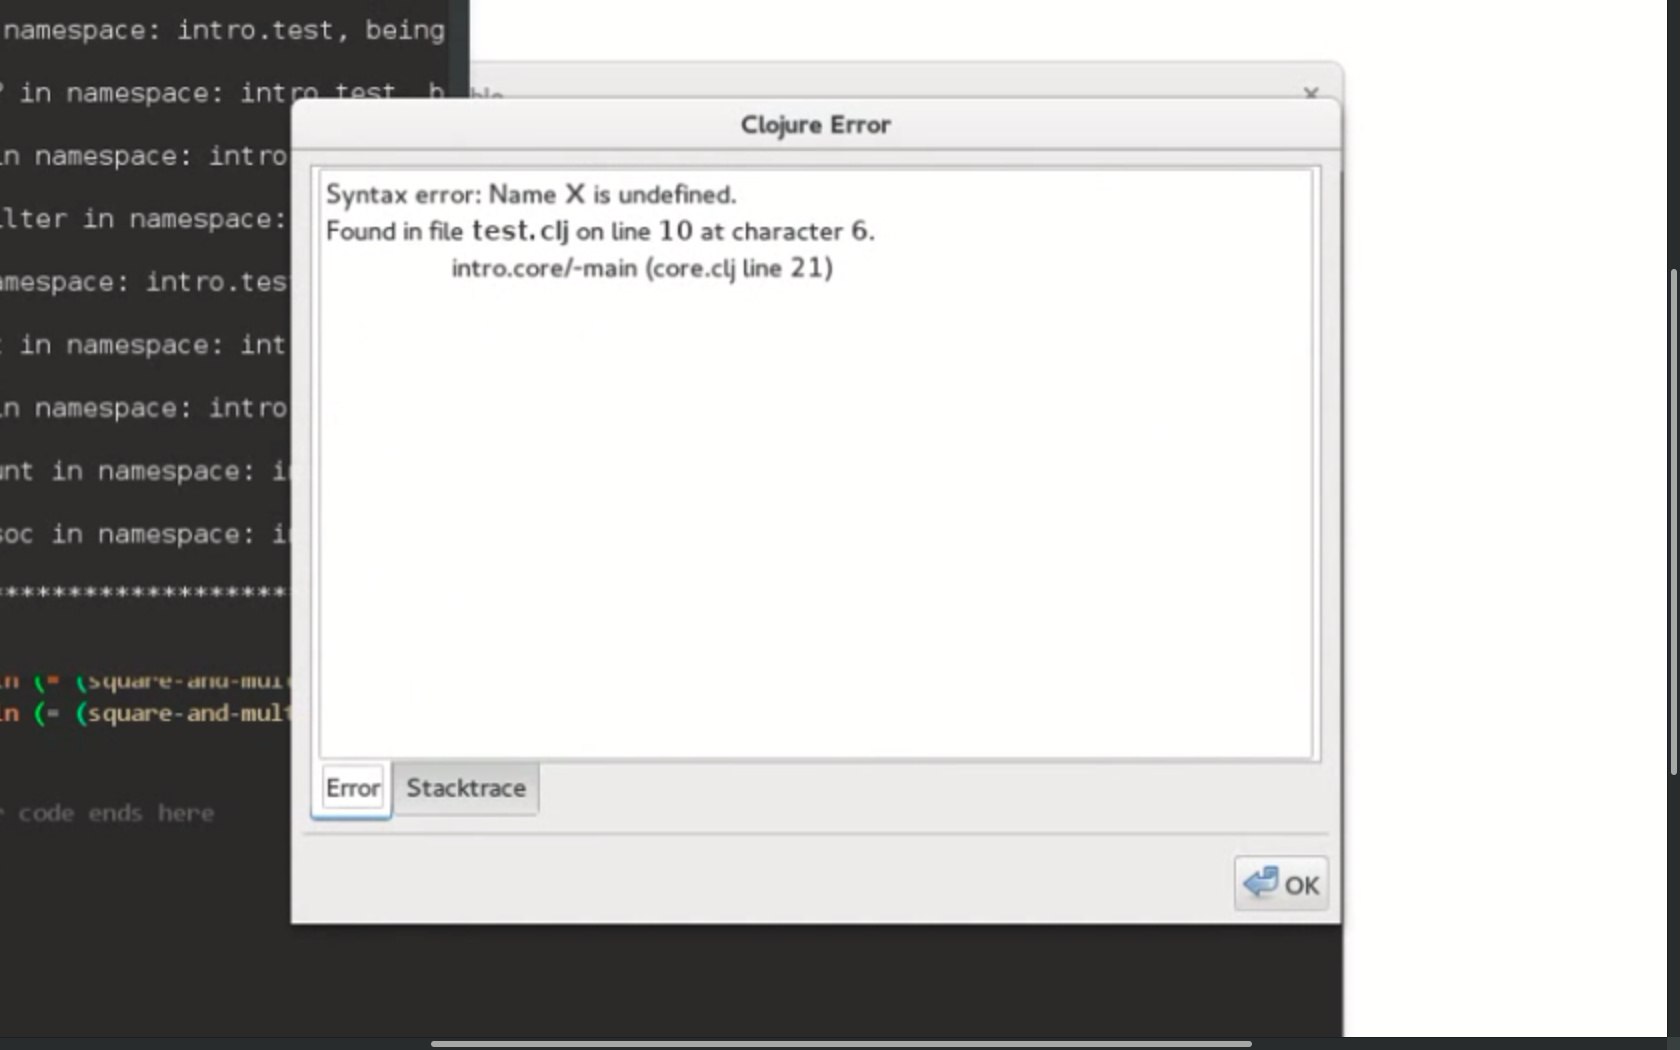
\includegraphics[scale=.17]{CM16shot}
\end{frame}

\begin{frame}
  \frametitle{Procedure}
\begin{itemize}

\item Generate Seed Number
\item Assign Racket \& Clojure Questions at Random
\item Randomly Assigned Group of either Clojure with Modified or Standard Error Messages
\item Record for 21 Minutes Racket, Optional Break Time, 21 Minute Clojure
\item Interview Questions
  
\end{itemize}  
\end{frame}

\begin{frame}
  \frametitle{Study Home Screen}
  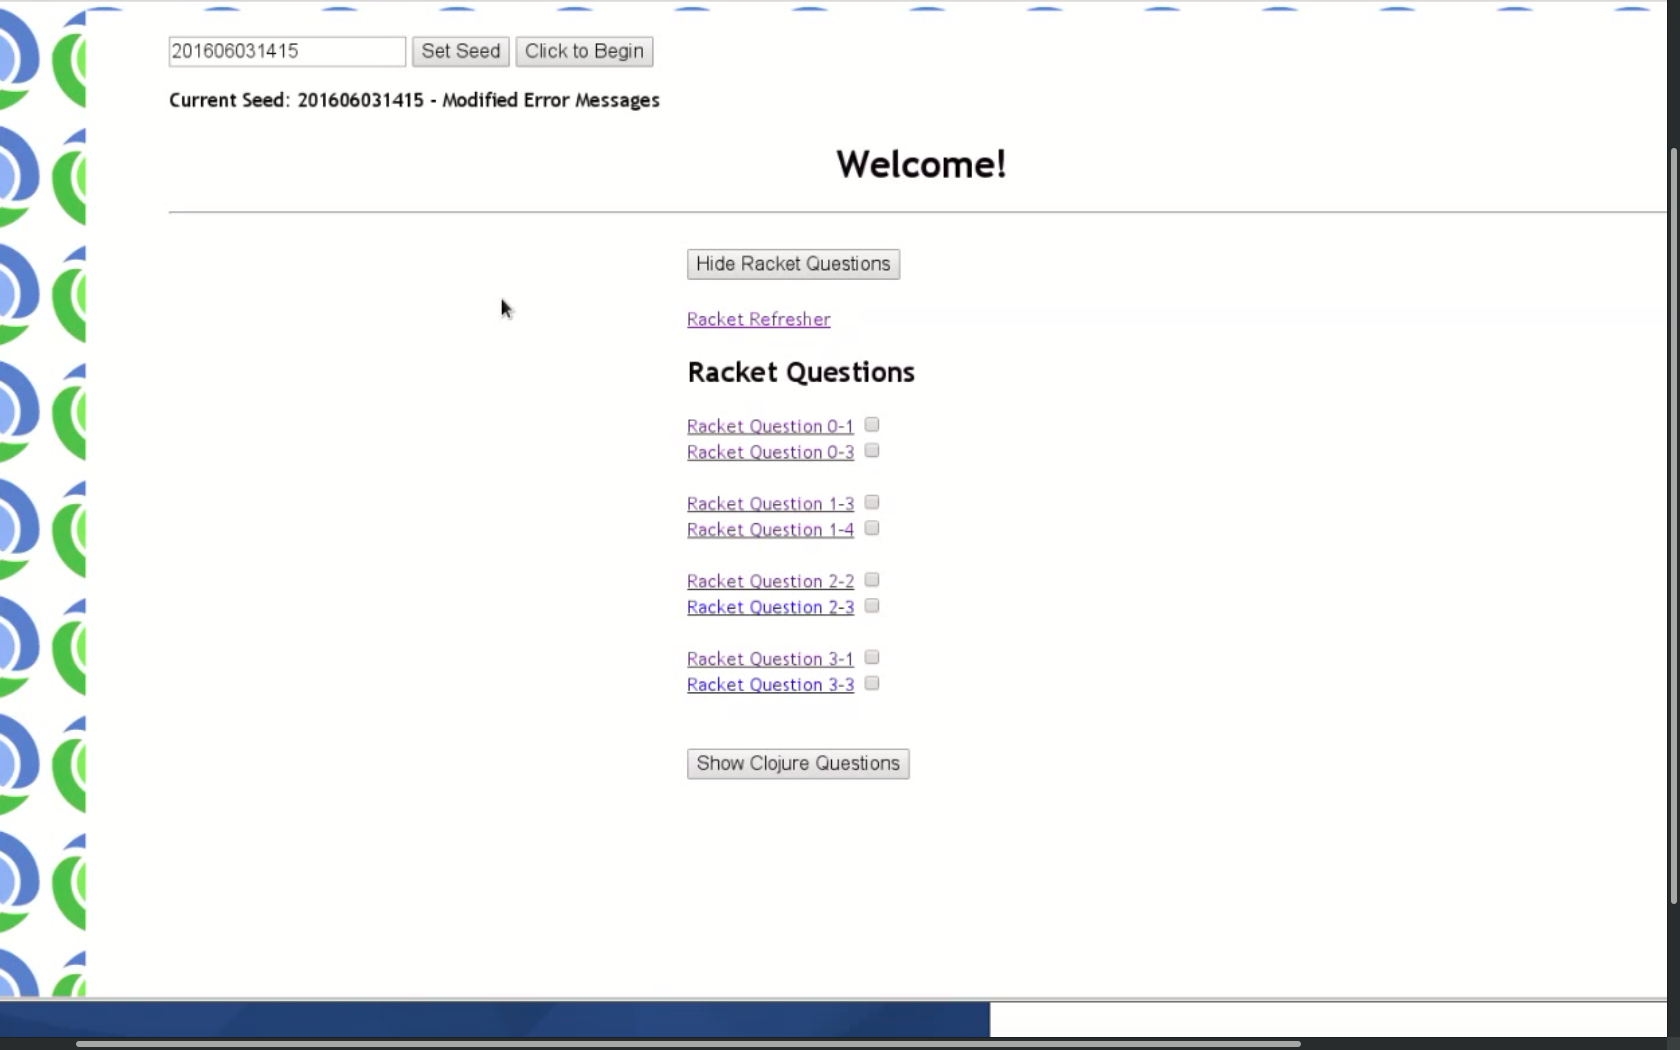
\includegraphics[scale=.17]{StudyHomeScreen}
\end{frame}

\begin{frame}
  \frametitle{Interview Questions}
 \begin{itemize}
 
\item What parts of the study were easy or clear to understand?
\item What parts of the study were difficult or confusing?
\item What would you suggest improving in the error messaging system in Racket or Clojure? 
 
 \end{itemize}
\end{frame}  




\section{Work in progress}

\begin{frame}
  \frametitle{Work in progress}
\begin{itemize}
\item Continued usability study 
\item Project re-structuring
\end{itemize}
\end{frame}

\begin{frame}
  \frametitle{Continued usability study }
More data points are needed for data analysis
\begin{figure}
%%% note: the file is in the same folder as your .tex file
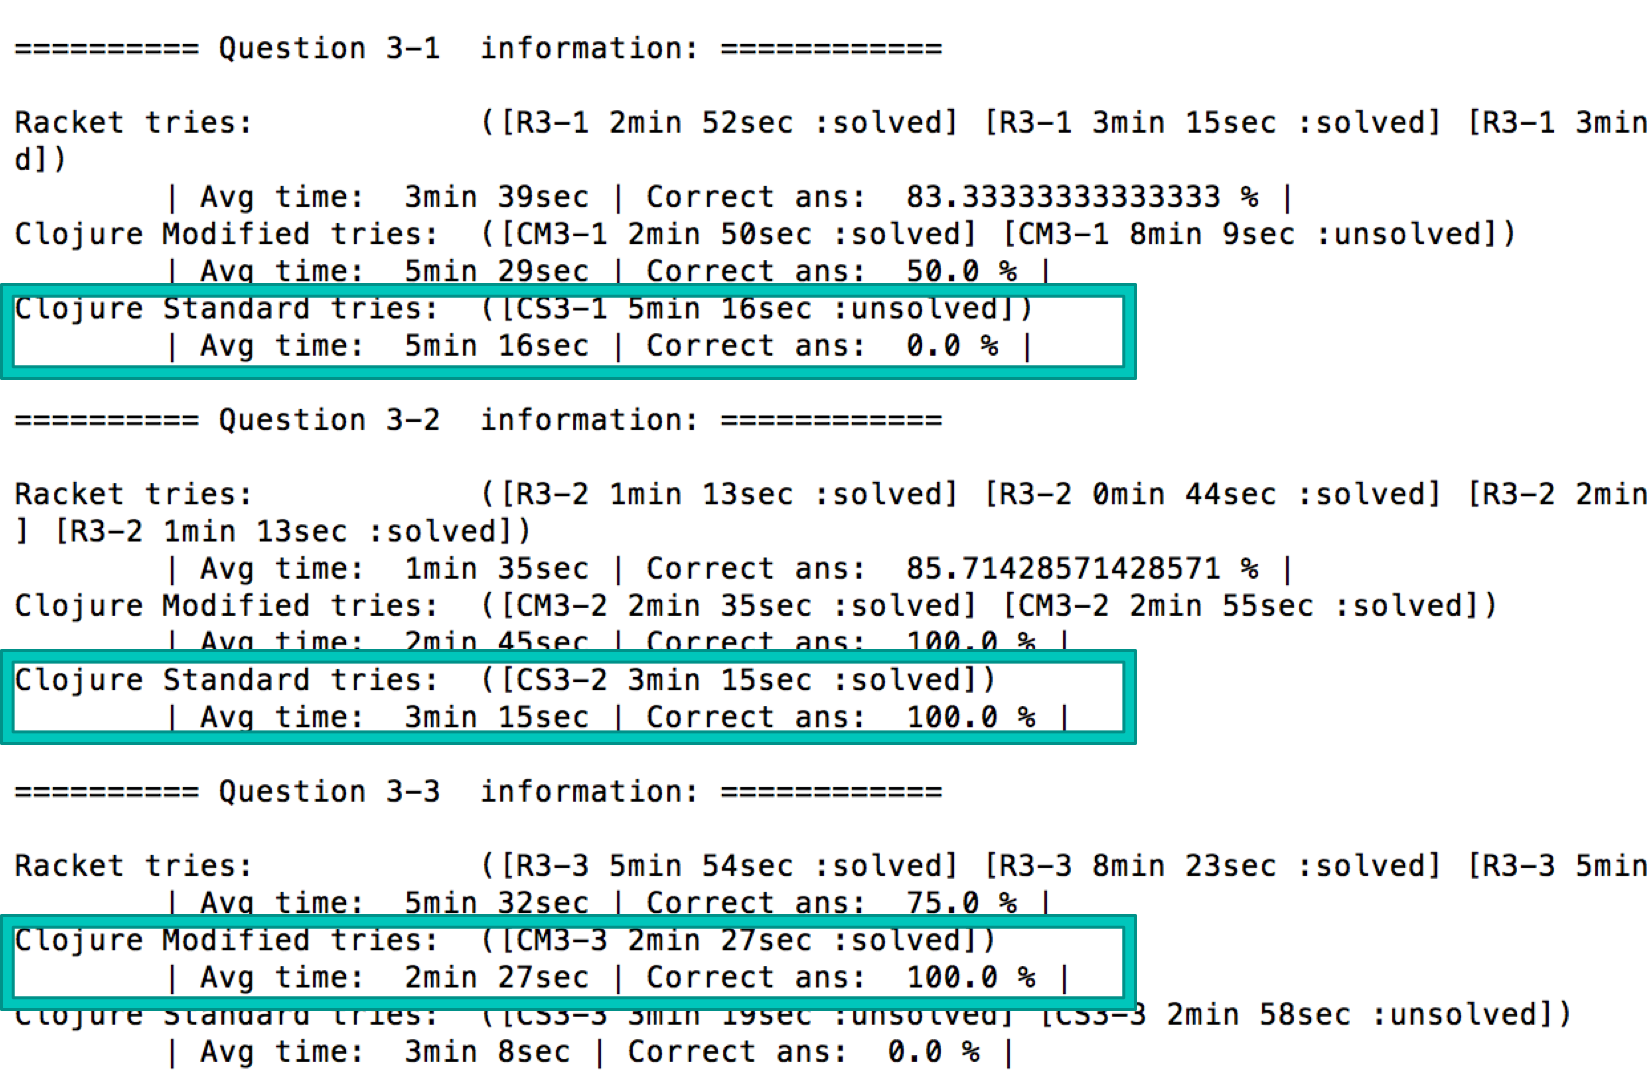
\includegraphics[height=55mm]{one-data.png}
\end{figure}
\end{frame}


\begin{frame}
  \frametitle{Project re-structuring}
How we handle when an error occurs 
\begin{figure}
%%% note: the file is in the same folder as your .tex file
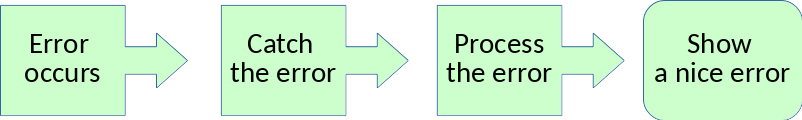
\includegraphics[height=15mm]{Step.png}
\end{figure}
\alert{Processing} is the most challenging part
\end{frame}


\begin{frame}
  \frametitle{Project re-structuring}
%Detailed explanation about atom processing
%The advantages of the new structure
Failing information is stored in a variable for processing
\begin{figure}
%%% note: the file is in the same folder as your .tex file
\includegraphics[height=40mm]{atom-ex.png}
\end{figure}
\end{frame}

\begin{frame}
  \frametitle{Project re-structuring}
The global variable is not used anymore
\begin{figure}
%%% note: the file is in the same folder as your .tex file
\includegraphics[height=20mm]{no-atom-ex.png}
\end{figure}
\end{frame}

\begin{frame}
  \frametitle{Discussion}
Questions?
\end{frame}

\end{document}

